% TODO fill in your paper title
\newcommand{\PaperTitle}{Remotely Mapping the World's Cell Towers}
% TODO fill in your paper number when you get it
\newcommand{\PaperNumber}{XXX}

% TODO specify your conference (ccs, imc, oakland, sigcomm, etc.)
\documentclass[usenix]{paper}

% This template file contains packages and commands that are useful and generic
% across papers.
%
% When adding new commands, you can most likely do that within paper.tex, but
% when adding new packages, you might need to update that here to ensure the
% packages are included in the proper order (a common source of compilation
% errors with LaTeX).

%%%%%%%%%%%%%%%%%%%%%%%%%%%%%%%%%%%%%%%%%%%%%%%%%%%%%%%%%%%%%%%%%%%%%%%%%%%%
% Packages {{{

\usepackage{color}
\ifieeeformat
\usepackage[dvipsnames]{xcolor} % IEEE needs this; ACM doesn't
\usepackage{totpages} % IEEE needs this; ACM doesn't
\fi
\usepackage{graphicx}
\graphicspath{{./figs/}}
\usepackage[labelformat=simple]{subcaption}
\usepackage{xspace}
\usepackage{multirow}
\usepackage{makecell} % Not sure if we need this
\ifieeeformat \else
\usepackage{enumitem} % Not sure if we need this
\fi
\usepackage[ruled,vlined]{algorithm2e}
\usepackage[nolist,nohyperlinks]{acronym}

\acrodefplural{BTS}[BTSes]{Base Station Transceivers}
\acrodefplural{CPS}[CPSes]{Cellular Positioning Systems}
\acrodefplural{WPS}[WPSes]{Wi-Fi Positioning Systems}

\usepackage{ulem}
\normalem

% }}}
%%%%%%%%%%%%%%%%%%%%%%%%%%%%%%%%%%%%%%%%%%%%%%%%%%%%%%%%%%%%%%%%%%%%%%%%%%%%
% Commands {{{

\newcommand{\etal}{et~al.\xspace}
\newcommand{\eg}{e.g.\xspace}
\newcommand{\ie}{i.e.\xspace}

\newcommand{\cps}{\ac{CPS}\xspace}
\newcommand{\wps}{\ac{WPS}\xspace}
\newcommand{\wifi}{Wi-Fi\xspace}

\newcommand{\cmark}{\ding{51}}%
\newcommand{\xmark}{\ding{55}}%

\renewcommand\thesubfigure{(\alph{subfigure}) }

\newcommand{\parhead}[1]{\medskip \noindent \textbf{#1}\hskip .1in}

% }}}
%%%%%%%%%%%%%%%%%%%%%%%%%%%%%%%%%%%%%%%%%%%%%%%%%%%%%%%%%%%%%%%%%%%%%%%%%%%%
% Environments {{{

\newenvironment{strategy}[1][htb]
  {\renewcommand{\algorithmcfname}{Strategy}
   \begin{algorithm}[#1]%
  }{
   \end{algorithm}
   }
  
\newenvironment{tightlist}{
	\begin{list}{$\bullet$} {
		\setlength{\itemsep}{0.00cm}
		\setlength{\parskip}{-0.1cm} 
	}}{\end{list}}

\newenvironment{widelist}{
	\begin{list}{$\bullet$} {
		\setlength{\leftmargin}{.70cm}
		\setlength{\itemsep}{.00cm}
	}}{\end{list}}

% }}}
%%%%%%%%%%%%%%%%%%%%%%%%%%%%%%%%%%%%%%%%%%%%%%%%%%%%%%%%%%%%%%%%%%%%%%%%%%%%
% Comment Commands {{{

\ifdefined\isFinalized
\newcommand{\NewCommentType}[3]{}
\else
\newcommand{\NewCommentType}[3]{\expandafter\newcommand\csname #1\endcsname[1]{{\color{#2}{#3: ##1}} }}
\fi

% }}}
%%%%%%%%%%%%%%%%%%%%%%%%%%%%%%%%%%%%%%%%%%%%%%%%%%%%%%%%%%%%%%%%%%%%%%%%%%%%
% Line-break nudging {{{

\clubpenalty=10000 
\widowpenalty = 10000 

\hyphenation{de-a-non-y-mi-za-tion}
\hyphenation{none-the-less}

% }}}
%%%%%%%%%%%%%%%%%%%%%%%%%%%%%%%%%%%%%%%%%%%%%%%%%%%%%%%%%%%%%%%%%%%%%%%%%%%%
% Prettier fonts {{{

\ifieeeformat \else
\urlstyle{tt}
\fi

\usepackage[override]{cmtt} % make tt font tighter / less ugly

% }}}
%%%%%%%%%%%%%%%%%%%%%%%%%%%%%%%%%%%%%%%%%%%%%%%%%%%%%%%%%%%%%%%%%%%%%%%%%%%%

\begin{document}

%%%%%%%%%%%%%%%%%%%%%%%%%%%%%%%%%%%%%%%%%%%%%%%%%%%%%%%%%%%%%%%%%%%%%%%%%%%%
% Paper-specific commands {{{

% System name (if applicable)
\newcommand{\name}{$\mathsf{SystemName}$\xspace} % middle of sentence
\newcommand{\Name}{$\mathsf{SystemName}$\xspace} % start of sentence

% Per-author comment commands (they don't appear if you "make finalized")
% 	Colors: black, blue, brown, cyan, darkgray, gray, green, lightgray, lime
% 	magenta, olive, orange, pink, purple, red, teal, violet, white,	yellow
\NewCommentType{todo}{red}{TODO}
\NewCommentType{dml}{violet}{dml}

% }}}
%%%%%%%%%%%%%%%%%%%%%%%%%%%%%%%%%%%%%%%%%%%%%%%%%%%%%%%%%%%%%%%%%%%%%%%%%%%%

\Abstract{abstract}

\input{intro}
\section{Background}
\label{sec:background}

\subsection{Positioning Systems}

\emph{Wireless positioning systems} are used by mobile operating systems to
compute their own locations. These systems use landmarks---either \wifi \acp{AP}
or cellular base stations---whose locations are known to provide devices
attempting to self-geolocate with reference points to use. 

\section{Related Work}
\label{sec:related}

Several smartphone applications have been developed to attempt to detect rogue
base stations. Park~\etal evaluated five popular IMSI catcher
applications---\emph{SnoopSnitch}~\cite{snoopsnitch}, \emph{Cell Spy Catcher},
\emph{GSM Spy Finder}, \emph{Darshak}~\cite{darshak}, and the \emph{Android IMSI
Catcher Detector (AIMSICD)}~\cite{AIMSICD},---for Android in order to evaluate
their efficacy against rogue base stations using a rogue base station framework
they developed called \emph{White-Stingray}~\cite{whitestingray}. Since this
work was published in 2017, several of these applications are no longer
available in the Google Play Store. 

More recently, Arnold~\etal, developed \emph{CellGuard}, an iOS application for
analyzing nearby cellular networks to detect possible rogue base
stations~\cite{cellguard}. \emph{CellGuard} uses several factors, including
whether or not a base station is present in Apple's \cps, to make this
determination. Unlike their work, which focuses on detecting a local adversary
in real time, this work seeks to map the world's cellular infrastructure and
detect malicious and suspicious rogue base stations longitudinally across time
and space.  

Most closely related to this work is Rye and Levin's investigation of the
security and privacy vulnerabilities associated with Apple's
\ac{WPS}~\cite{rye2024surveilling}. The authors demonstrated that an
unprivileged attacker can amass hundreds of millions of \wifi \ac{BSSID}
geolocations by querying Apple's \ac{WPS} with little \emph{a priori} knowledge.
In this work, we 

\section{Methodology}
\label{sec:methodology}

This section details our methodology for geolocating cellular infrastructure
using Apple's \ac{CPS}. 

\begin{table}[t]
    \centering
    \caption{OpenCelliD \ac{BTS} counts by cellular generation from March 2025.}
    \label{tab:opencellid-counts}
    \begin{tabular}{c|r}
    \textbf{Technology} & \multicolumn{1}{|c}{\textbf{Count}} \\
    \hline
    GSM & 1,300,596  \\
    UMTS & 473,432 \\
    CDMA & 28 \\
    LTE & 2,726,803 \\
    NR & 120,009  \\
    \hline
    Total & 4,620,869
    \end{tabular}
\end{table}


\subsection{Bootstrapping \acp{BTS}}

Apple's \ac{CPS} requires Apple devices to submit the unique identifiers of
nearby \acp{BTS} in order to receive their geolocations. However, beyond the
\ac{PLMN}, which identifies an \ac{MNO}, there is no universal structure or
format for how cells are numbered. Doing so is left up to individual \acp{MNO},
and their numbering plan may vary substantially from other \acp{MNO}, even
within the same country. Further, because the combined location and cell
identifier address spaces range from 28 to 32 bits, depending on the technology
(\ref{tab:cellids}), guessing within or exhaustively enumerating the identifier
space is an inefficient way to accumulate geolocated cell data.

This presents a chicken and egg problem---how might one gather a baseline of
geolocated \ac{BTS} data to bootstrap the geolocation? To solve this dilemma, we
turned to a free database provided by OpenCelliD~\cite{opencellid}. OpenCelliD
provides worldwide, geolocated \ac{BTS} data for free

\section{Results}
\label{sec:results}


\begin{table}[t]
    \centering
    \caption{Base station counts by cellular technology.}
    \label{tab:generation-counts}
    \begin{tabular}{c|r}
    \textbf{Technology} & \multicolumn{1}{|c}{\textbf{Count}} \\
    \hline
    GSM/UMTS            & 36,041,875                         \\
    LTE                 & 48,107,561                         \\
    NR                  & 2,891,114                          \\
    \hline
    Total               & 87,040,550                        
    \end{tabular}
\end{table}

\section{Case Studies}
\label{sec:casestudies}

\begin{figure*}[t]
    \centering
    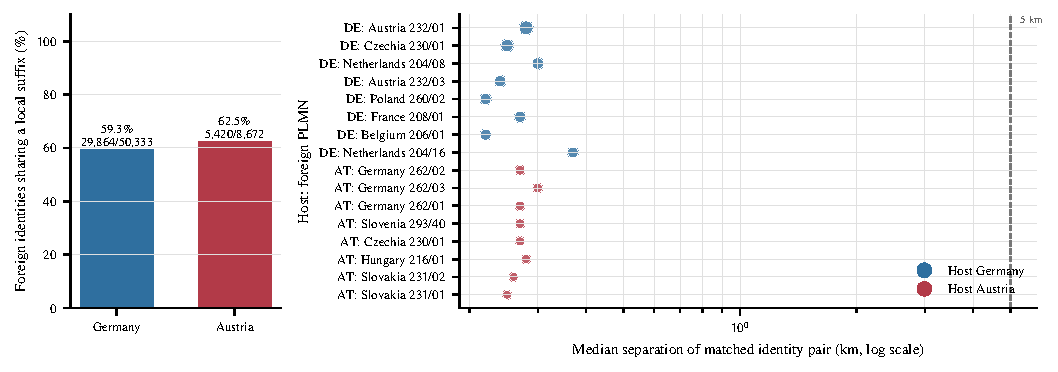
\includegraphics[width=\linewidth]{germany_austria_aliasing_diagnostic.pdf}
    \caption{A majority of foreign identities in Germany and Austria share local identifier suffixes, and the sub-kilometer separation of matched pairs supports identifier aliasing.}
    \label{fig:germany-austria-aliasing}
\end{figure*}

\begin{figure*}[t]
    \centering
    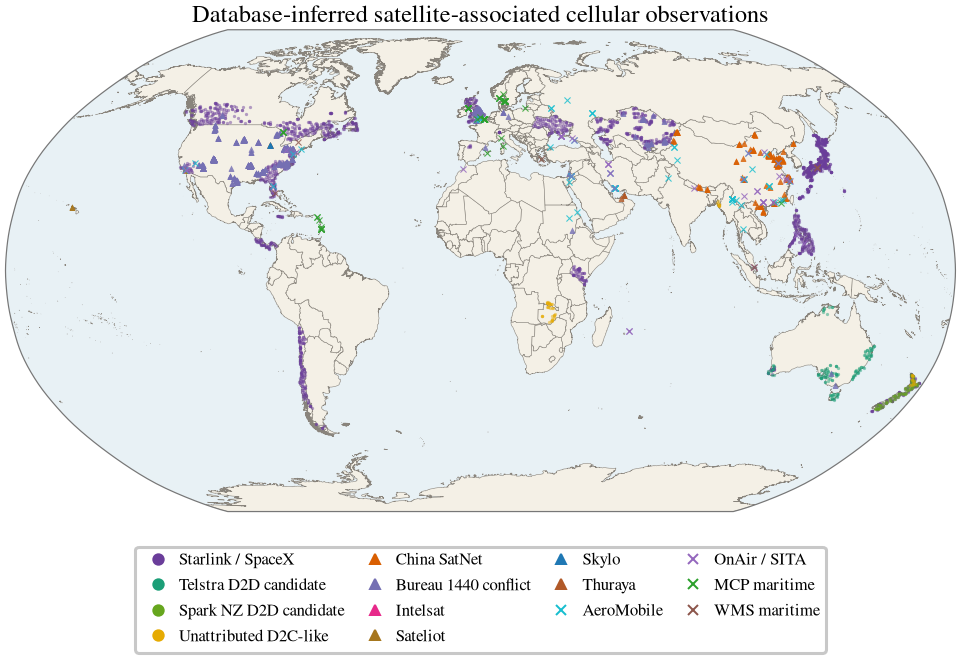
\includegraphics[width=\linewidth]{satellite_world_map.pdf}
    \caption{Satellite-associated cellular observations combine TAC centroids for D2C-like populations with sparse directly assigned and onboard-network locations, while all Starlink and SpaceX observations share one category.}
    \label{fig:satellite-world-map}
\end{figure*}

\begin{figure*}[t]
    \centering
    \setlength{\tabcolsep}{1pt}
    \begin{tabular}{cccc}
        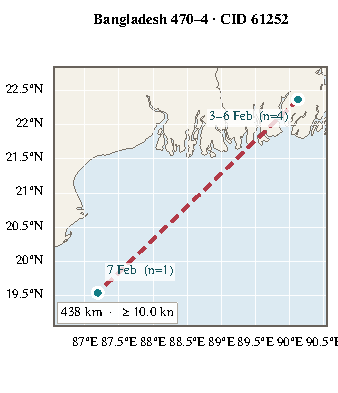
\includegraphics[width=0.245\linewidth]{ocean_vessel_banglalink.pdf} &
        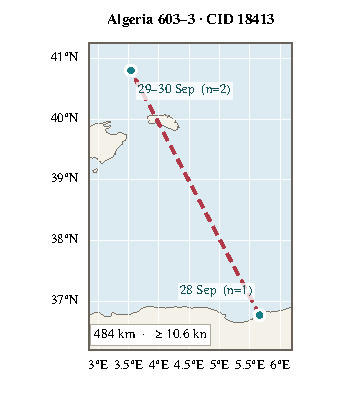
\includegraphics[width=0.245\linewidth]{ocean_vessel_algeria_18413.pdf} &
        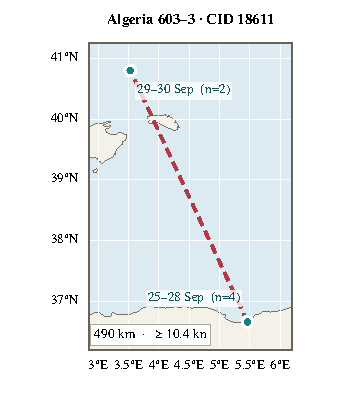
\includegraphics[width=0.245\linewidth]{ocean_vessel_algeria_18611.pdf} &
        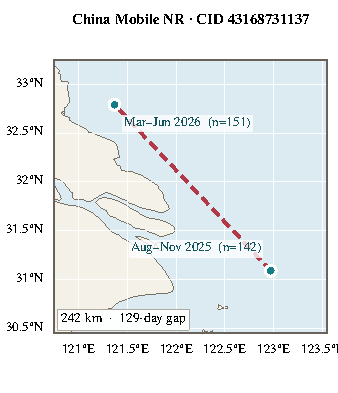
\includegraphics[width=0.245\linewidth]{ocean_vessel_china_nr_relocation.pdf}
    \end{tabular}
    \caption{Large offshore coordinate changes comprise three temporally plausible vessel-carried GSM candidates and one repeatedly supported China Mobile NR relocation separated by a 129-day observation gap.}
    \label{fig:ocean-vessel-movements}
\end{figure*}

\subsection{Moving Base Stations}

\begin{figure*}[t]
    \centering
    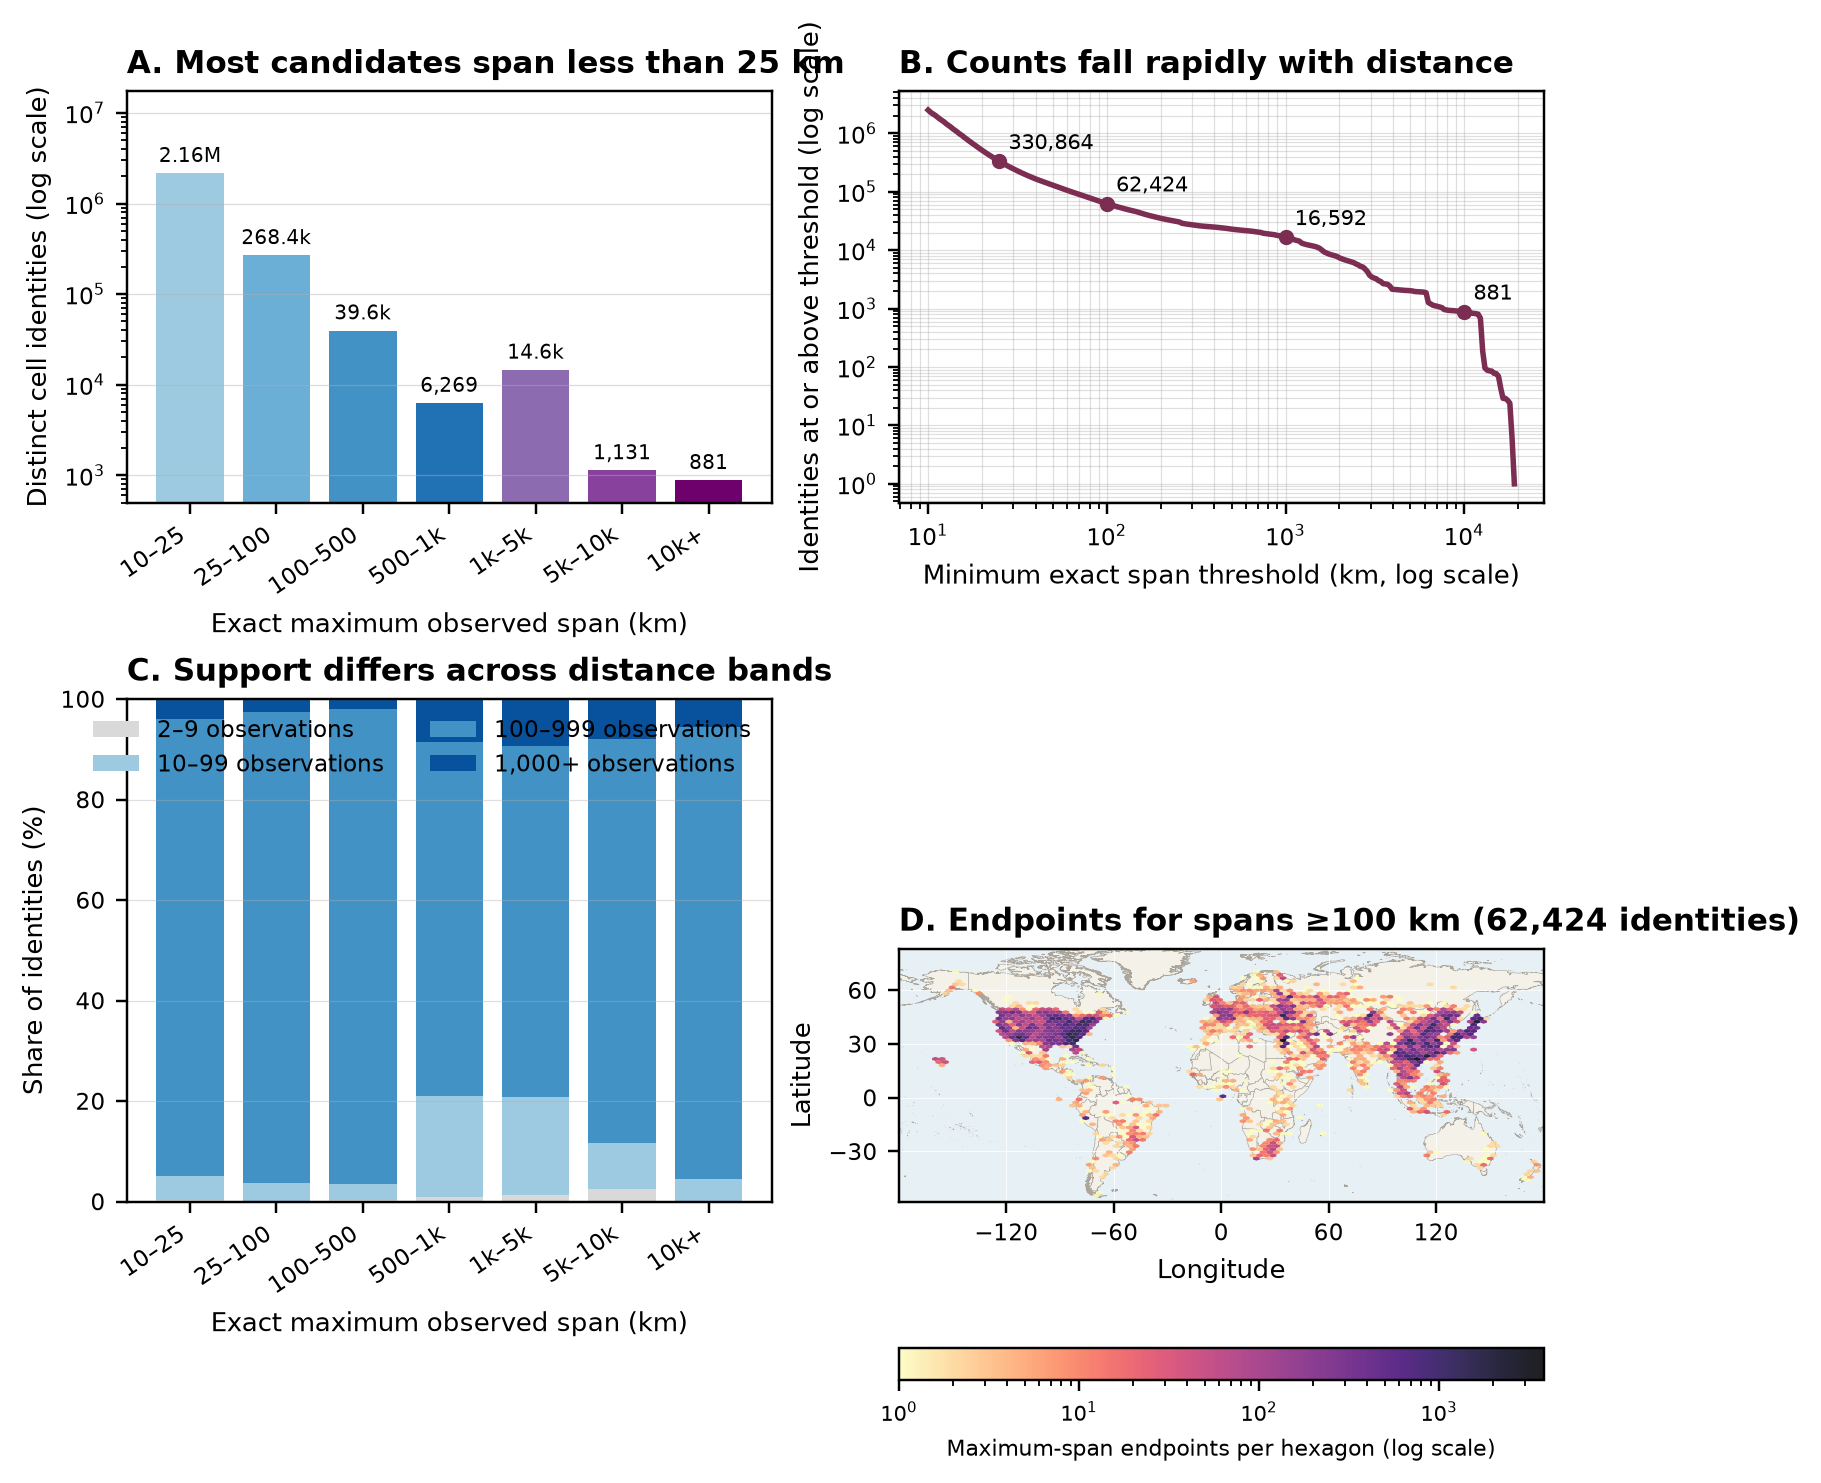
\includegraphics[width=\linewidth]{moving_mccs_overview.pdf}
    \caption{Among cell identities with an exact observed span over 10\,km, most movements are short, while longer-distance endpoints are globally distributed and vary substantially in observation support.}
    \label{fig:moving-mccs-overview}
\end{figure*}

\input{conclusion}

%%%%%%%%%%%%%%%%%%%%%%%%%%%%%%%%%%%%%%%%%%%%%%%%%%%%%%%%%%%%%%%%%%%%%%%%%%%%

%\bibliographystyle{plain}
\bibliography{conferences,refs}

\begin{acronym}
    \acro{AP}{access point}
    \acro{AKM}{Authentication and Key Management}
    \acro{BSSID}{Basic Service Set Identifier}
    \acro{ESS}{Extended Service Set}
    \acro{CPE}{Customer Premises Equipment}
    \acro{CPS}{Cellular Positioning System}
    \acro{EAP}{Extensible Authentication Protocol}
    \acro{ISP}{Internet Service Provider}
    \acro{PSK}{Pre-Shared Key}
    \acro{LAN}{Local Area Network}
    \acro{MAC}{Media Access Control}
    \acro{OUI}{Organizationally Unique Identifier}
    \acro{WLAN}{Wireless Local Area Network}
    \acro{WPS}{Wi-Fi Positioning System}
\end{acronym}


\end{document}
